\documentclass{article}
\usepackage[utf8]{inputenc}

\title{Systematically Providing Descriptive Names for Unit Tests \\ 
Ph.D. Dissertation Proposal}
\author{\textbf{Jianwei Wu} \\
\small wjwcis@udel.edu}
\date{Nov 2019 - 2020}

\usepackage{natbib}
\usepackage{graphicx}
\usepackage{csquotes}
\usepackage{siunitx}
\usepackage{booktabs}
\usepackage{cleveref}

\begin{document}

\maketitle

\tableofcontents

\section{Introduction}

~~The overall topic of the dissertation is about solving the naming problem in unit testing.
%
The first part we investigated is about improving non-descriptive test names.
%
The second part we will develop is a learning-based\slash graph-based technique to globally provide descriptive test names since the naming of tests is not \enquote{local}.
%
The last part we will develop is a comprehensive study that can provide descriptive names for every code element in unit tests (i.e., identifiers, test names, test class names, etc.).


\begin{itemize}
	\item First Section: improving test names.
	\item Second Section: globally predict descriptive test names.
	\item Third Section: comprehensively provide descriptive names for unit testing.
\end{itemize}

\section{A Pattern-based Approach to Detect and Improve Non-descriptive Test Names}

...


\section{A Concept-based Approach to Globally Provide Descriptive Test Names}


\subsection{Motivation}

\begin{table*}
\centering
\begin{tabular}{
  l
  l
  S[table-format=5]
}
 \toprule 
 \multicolumn{1}{c}{\textbf{Project}} & \multicolumn{1}{c}{\textbf{Commit}} & \multicolumn{1}{c}{\textbf{\# Renames}} \\
 \midrule
 Picasso    & 5c05678 & 22  \\
 mockito    & 2204944 & 112 \\
 Guice      & 6f1c6cc & 7   \\
 fastjson   & 4c7935c & 62  \\
 Guava      & bf4627d & 165 \\
 ExoPlayer  & c02f3dd & 44  \\ 
 \midrule
 \multicolumn{2}{r}{Total} & 412 \\
 \bottomrule
\end{tabular}
\caption{Preliminary Subjects.}
\label{tab:subjects}
\end{table*}

\begin{figure}[t]
    \centering
    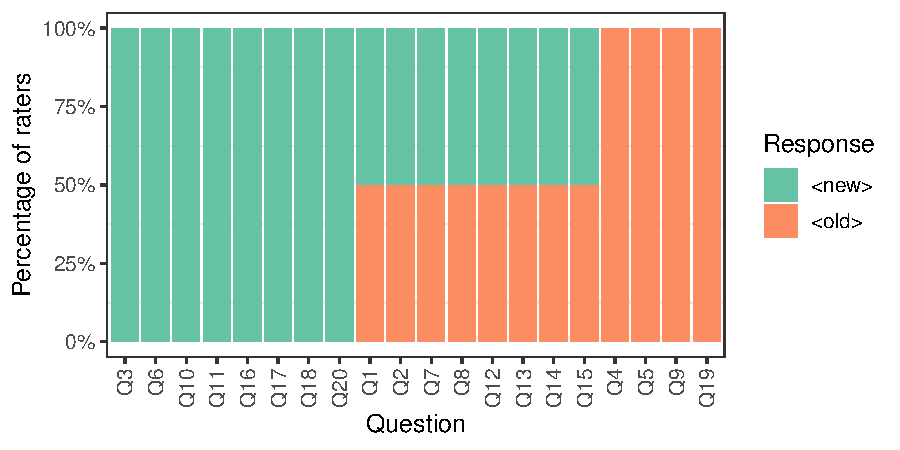
\includegraphics[scale=0.5]{./plots/motivation_plot.pdf}
    \caption{Survey Results.}
    \label{fig:prelim_survey}
\end{figure}


The motivation section is composed of a pilot survey and a basic analysis using \textit{Code2Seq}~\cite{alon2018code2seq}.
%
As the first step of this paper, we first investigated six projects as the preliminary subjects that are built for different purposes: new collections' library, media player, mocking framework, and so on.
%
In~\cref{tab:subjects}, the first column is the name of the project, the second column is the commit hash for the specific version of the project, and the last column is showing the number of renames that each project has.
%
For example, the \textit{ExoPlayer} project has \num{44} tests that are renamed during the process of developing the project.


For the pilot survey, we automatically generated a pilot survey with 21 questions.
%
The first part of the survey contains 20 questions, each question showed the recipient a test body with two test names and asked them to choose a test name that he/she think is better.
%
Moreover, in the pilot survey, all test bodies with their renames are randomly chosen from the \num{412} renames in~\cref{tab:subjects}.
%
The last question was asking their choosing strategies as a text entry.
%
From the survey results in~\cref{fig:prelim_survey}, we can see that \num{60}\% of new names are chosen in the results produced by the two recipients that we invited for the pilot survey.
%
Reviewing from the results of the pilot survey, it shows the renaming of a test name should be caused by a change of the test body or an attempt to improve current test name, and the new names are generally better the old names (i.e., more descriptive).


For the basic analysis, we utilized a state-of-the-art tool based on machine learning - \textit{Code2Seq} to make prediction of test name for each test contained in the preliminary subjects.
%
After we gathered \num{14183} valid predicted names from \textit{Code2Seq}, a basic data analysis was performed on those predicted names to find duplicated predictions within their corresponding test classes.
%
From our preliminary analysis, there are \num{2124} duplicates in the predicted test names.
%
The average number of duplicated names per project is \num{354}, and the average number of duplicated names per test class is roughly \num{1.2}.
%
Even with a state-of-the-art tool, it still produces test names that are locally predicted rather than globally due to the existence of duplication.
%
In this paper, we propose a concept-based approach to globally provide descriptive test names by using formal concept analysis (FCA)~\cite{tonella2004formal}.



123



\section{Remaining Work}

    
\subsection{A Comprehensive Approach to Provide Descriptive Names for Every Code Element in Unit Testing or Automatically Generate Descriptive Summary\slash User's Manual for Open-source Project}


\section{Foreseen Contributions}



...


% \section{Solving the Naming Problem v2}

% The overall topic of the dissertation is about solving the naming problem in different parts of program.
% %
% The first part we investigated is about improving non-descriptive test names.
% %
% The second part we will investigate is to find the method and class names that are renamed for multiple times.
% %
% The last part we will develop is to combine those two techniques to generating human-readable test names.

% \begin{itemize}
% 	\item First Section: improving test names.
% 	\item Second Section: finding test names that are renamed for multiple time.
% 	\item Third Section: generating human-readable test names.
% \end{itemize}

% \subsection{Detect and Improve Non-descriptive Test Names}

% ...

% \subsection{Finding Potential Problematic Test Names}

% ...

% \subsection{Generating Human-readable Test Names by Combine Pattern and Rename Logs}

% ...

\bibliographystyle{plain}
\bibliography{proposal}
\end{document}
